\documentclass{beamer}
\usepackage{graphicx}
\usepackage{listings}
\usepackage{beamerthemesplit}
\usetheme{Warsaw}

\title{Moogle!, ligth fast searching}
\author{Víctor Vena}
\date{16 de julio de 2023}



\begin{document}

\begin{titlepage}

   \begin{center}
    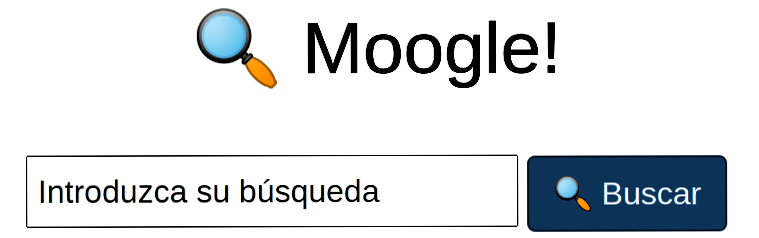
\includegraphics[scale=0.25]{Imagenes/moogle.png}
   \end{center}

\end{titlepage}

\centering

\section{Qué es Moogle!}

\begin{frame}{Qué es Moogle!}
    Moogle! es un motor de búsqueda con una interfaz amigable basada en web y búsquedas ligth fast.    
\end{frame}


\section{Características}

\subsection{Características}

\begin{frame}{Características}

    \begin{itemize}
        \item<1-> Búsquedas rápidas. Ofreciendo resultados al momento.
        \item<2-> Búsquedas inteligentes:
        \begin{itemize}
            \item<3-> Determina los términos más relevantes y prioriza los documentos que los contienen.
            \item<4-> Muestra los resultados más importantes primero.
        \end{itemize}
        \item<5-> Muestra fragmentos de los documentos.
        \item<6-> Ofrece alternativas ante palabras mal escritas o que dan pocos resultados.
        \item<7-> Operadores para controlar el comportamiento de la búsqueda.
    \end{itemize}

\end{frame}

\subsection{Ejemplos}

\begin{frame}{Operadores}
    Usando operadores los operadores \^{} y !\\
    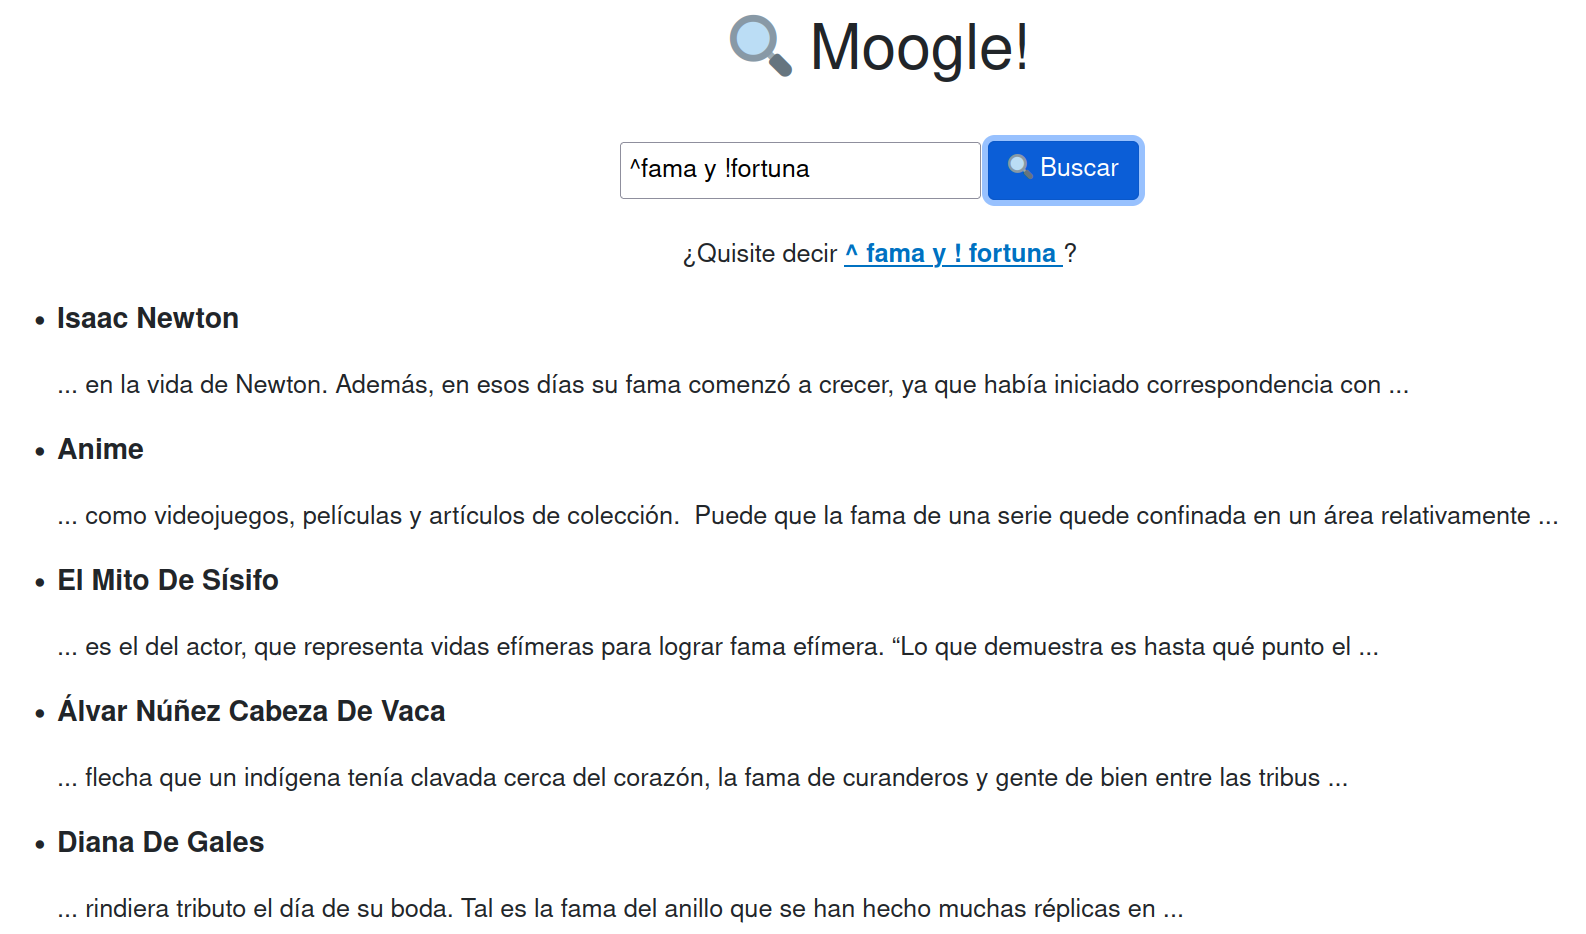
\includegraphics[scale=0.2]{Imagenes/Operadores1.png}
\end{frame}

\begin{frame}{Operadores}
    Sin usar el operador \~{}\\
    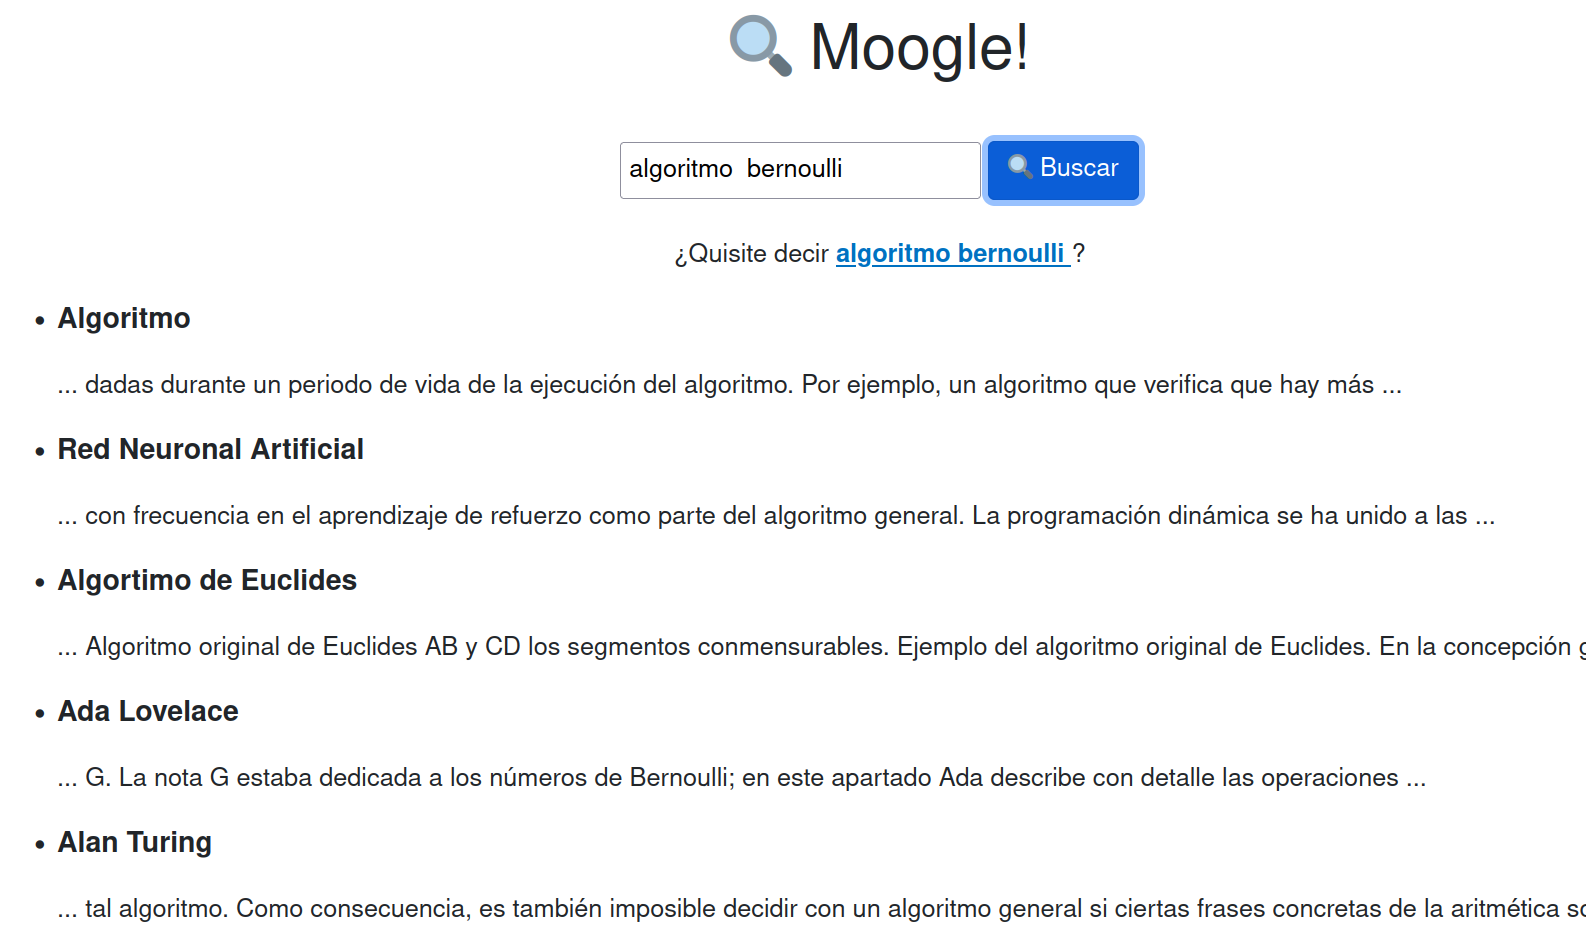
\includegraphics[scale=0.2]{Imagenes/Operadores2.png}
\end{frame}
\begin{frame}{Operadores}
    Usando el operador \~{}\\
    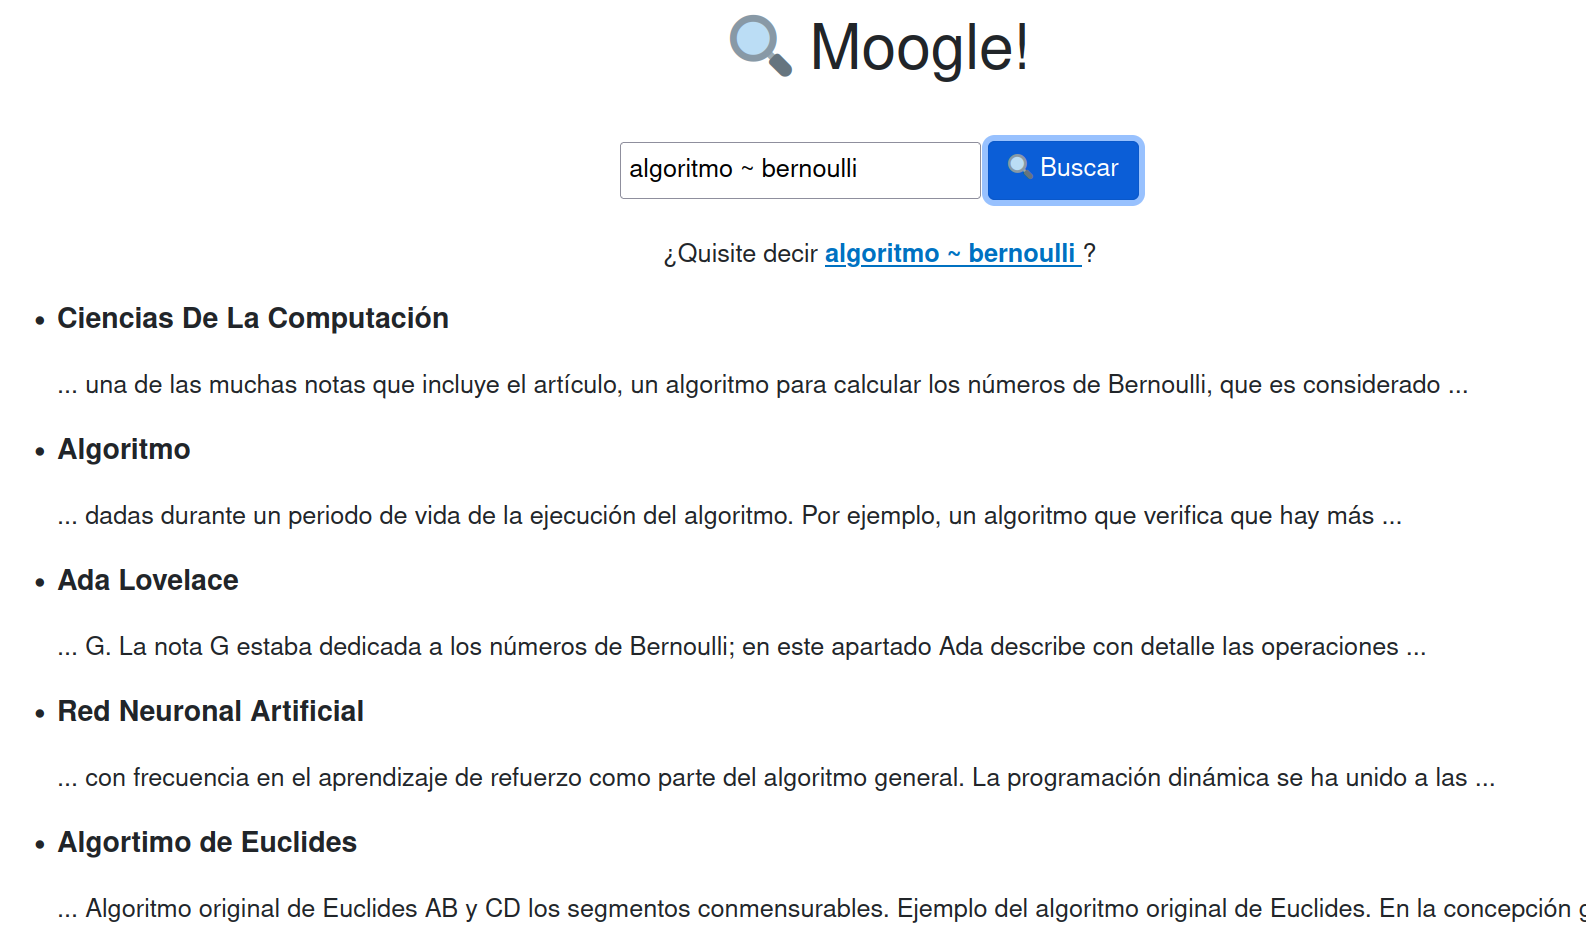
\includegraphics[scale=0.2]{Imagenes/Operadores3.png}
\end{frame}

\begin{frame}{Operadores}
    Tambien puedes hacer una sopa de operadores\\
    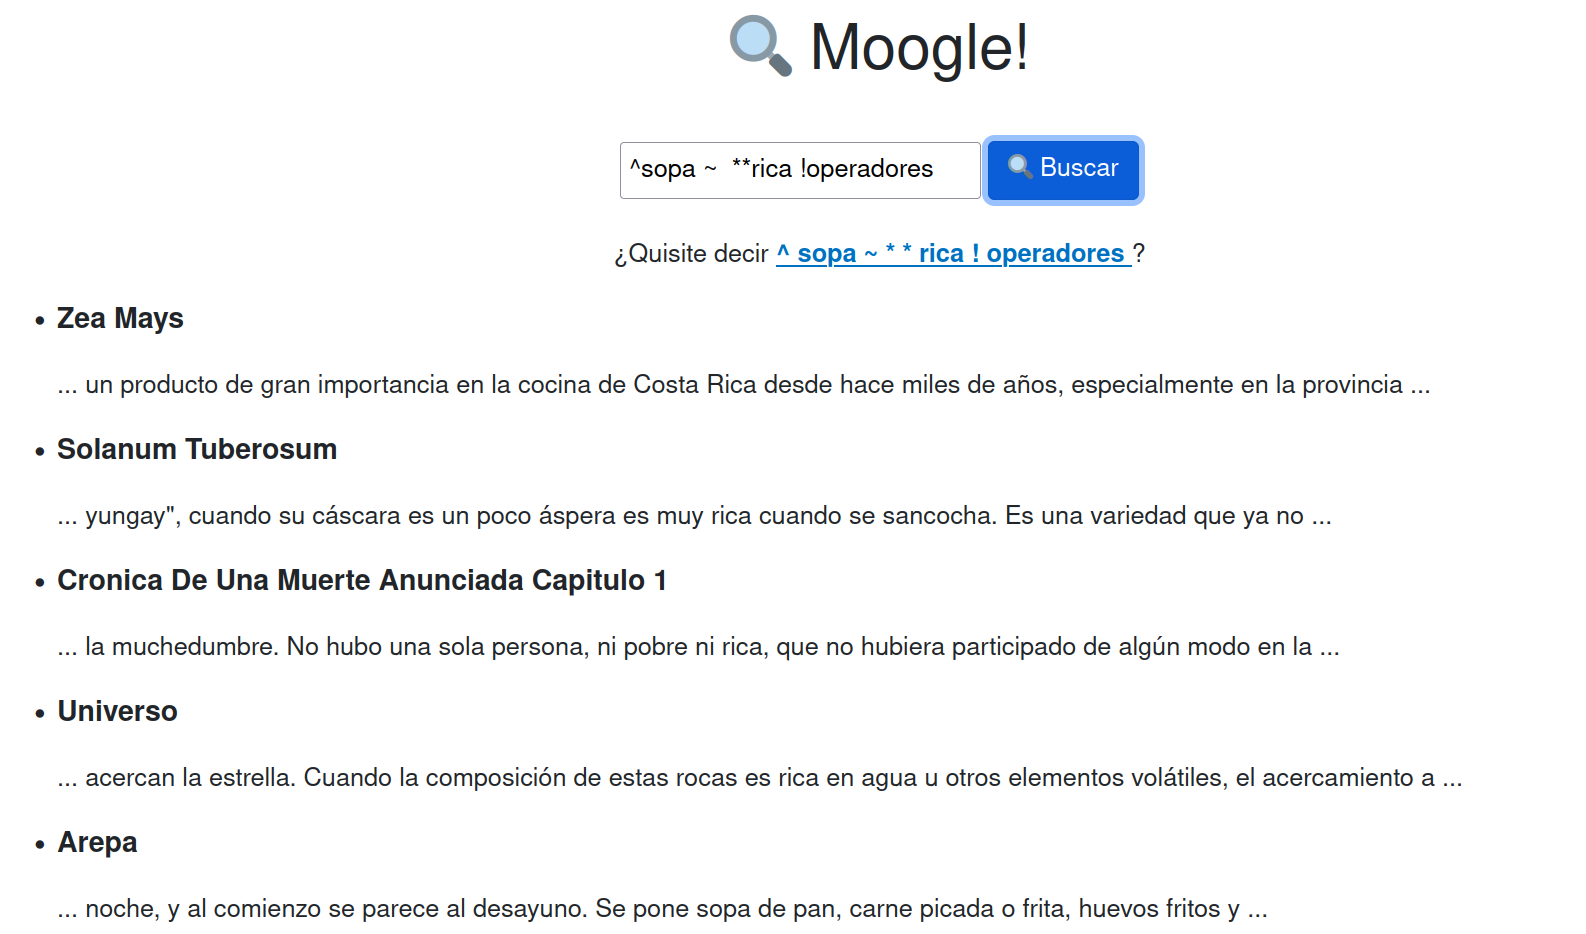
\includegraphics[scale = 0.2]{Imagenes/Operadores4.png}
\end{frame}

\begin{frame}{Operadores}
    Entendemos lo que quisiste decir\\
    \bigskip
    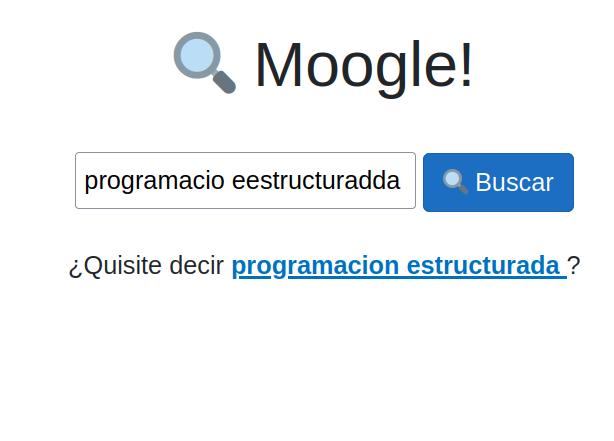
\includegraphics[scale=0.2]{Imagenes/programacion_estructurada.png}
\end{frame}

\section{Proximamente}

\begin{frame}{Proximamente}
    Posibilidad de configurar Moogle! para que realice las búsquedas en cualquier directorio que se desee.\\
\end{frame}


\section{Despedida}

\begin{frame}{The End \^{}\_\^{}}
    Esto es todo,disfruten usando Moogle!
\end{frame}

\end{document}